\documentclass[a4paper,11pt]{report}
%\usepackage[utf8]{inputenc}



%\usepackage[justification=centerlast,font=small]{caption}
\usepackage[T1]{fontenc}

% amssymb musi być przed \usepackage[polish]{babel}
% żeby nie było błędu ``command \lll already defined''
\usepackage{amssymb} 
                     
\usepackage[polish]{babel}
\usepackage{polski}

%\usepackage[utf8]{inputenc}
\usepackage{wrapfig}
%\usepackage{dirtytalk}
%\usepackage[demo]{graphicx}
\usepackage{siunitx}
\usepackage{textcomp}
\usepackage{icomma}
\usepackage{threeparttable}
\usepackage{graphicx}
\usepackage{subfig}
\usepackage{setspace}
%\usepackage{pdflscape}
\usepackage[paper=portrait,pagesize]{typearea} % dla stron obróconych
%% dla malych arrow
\usepackage{stmaryrd}
\newcolumntype{C}{>{\centering\arraybackslash}X}
\usepackage{longtable}
\usepackage{gensymb}
%\usepackage{hyperref}

% podpis tabeli nad tabelą
\usepackage{floatrow}
\floatstyle{plaintop}
\restylefloat{table}

%\usepackage[utf8x]{inputenc}  %%% TO POWODUJE BLAD NA OVERLEAF
\usepackage[bottom]{footmisc}
\usepackage[figurename=Fig.]{caption}
%\usepackage[section]{placeins}
\usepackage{color, soul} % highlighting
\newcolumntype{Y}{>{\centering\arraybackslash}X} %necessary for tabularx to make equal width columns
\usepackage[usenames,dvipsnames]{xcolor} 
%\newcommand{\hlc}[2][yellow]{ {\sethlcolor{#1} \hl{#2}} }
%\usepackage{graphicx} % for improved inclusion of graphics
%\usepackage{epstopdf}
%\usepackage{indentfirst} % wstawia wciecie w pierwszym akapicie rozdzia³u 
%\usepackage{amsfonts} % for \mathbf
%\usepackage{datetime}%zeby miec godzine kompilacji (opcja \date i \currenttime)
\usepackage{tabularx}%do robienia tabel
\usepackage{float}
\usepackage{amsmath}
%\usepackage{subcaption}
\usepackage{multirow}
\usepackage{booktabs}
\selectlanguage{polish}
%%%%%%%%%%%%%%%%%%%%%%% to prevent hyphenation %%%%%%%%%%%%%%%%%%%%%%%
%\usepackage[polish=nohyphenation]{hyphsubst}
\tolerance=1
\emergencystretch=\maxdimen
\hyphenpenalty=10000
\hbadness=10000
%\hyphenation{sze-regowo}
%%%%%%%%%%%%%%%%%%%%%%% end of to prevent hyphenation %%%%%%%%%%%%%%%%%%%%%%%
\usepackage{caption}% zamienia Rysunek na Rys. w podpisach rysunków
\captionsetup{figurename=Rys.}
\captionsetup{tablename=Tab.}
\captionsetup[table]{labelsep=space} % removes colon from caption
\captionsetup[figure]{labelsep=space} % removes colon from caption
% Zdefiniowanie autora i~tytułu:
\frenchspacing %wyłączenie wstawiania wiêkszych odstêpów na koñcu zdañ
\addtolength{\hoffset}{-0.5cm}
\addtolength{\textwidth}{1.0cm}%zwieksza szer. szpalty o liczbe cm
\usepackage{fancyhdr} %wstawia naglowki na stronach
%\pagestyle{headings}

%\pagestyle{fancy}
%\fancyhf{}
%\fancyhead[LE]{\leftmark}
%\fancyhead[RO]{\rightmark}
%\fancyfoot[LE,RO]{\thepage}
%\fancypagestyle{plain}{\fancyhf{}\fancyfoot[R]{\thepage}\renewcommand{\headrulewidth}{0pt}}
%\setlength{\headheight}{26pt}
%\usepackage[draft]{todonotes}   % notes showed; should be after xcolor

% do kolorowania pojedynczych komórek w tabelach \cellcolor
\usepackage{xcolor,colortbl}

\setcounter{tocdepth}{3} %%%% wyrzuca subsubsections z toc
\usepackage[most]{tcolorbox} % do rysowania kolorowych ramek z tekstem
\usepackage{hyperref}%do hiperłączy; powinno być jako ostatnie w preambule
%\hypersetup{colorlinks=false}%sprawia że kolorowe ramki hiperłączy nie są drukowane
\hypersetup{colorlinks,citecolor=black,filecolor=black,linkcolor=black,urlcolor=red}%wyłącza kolorowe ramki hiperłączy; linkiw www sa na czerwono

\usepackage{listings}
\usepackage{xcolor}
\usepackage{indentfirst} % wciecie akapitu

%New colors defined below
\definecolor{codegreen}{rgb}{0,0.6,0}
\definecolor{codegray}{rgb}{0.5,0.5,0.5}
\definecolor{codepurple}{rgb}{0.58,0,0.82}
\definecolor{backcolour}{rgb}{0.95,0.95,0.92}

%Code listing style named "mystyle"
\lstdefinestyle{mystyle}{
  backgroundcolor=\color{backcolour},   commentstyle=\color{codegreen},
  keywordstyle=\color{magenta},
  numberstyle=\tiny\color{codegray},
  stringstyle=\color{codepurple},
  basicstyle=\ttfamily\footnotesize,
  breakatwhitespace=false,         
  breaklines=true,                 
  captionpos=b,                    
  keepspaces=true,                 
  numbers=left,                    
  numbersep=5pt,                  
  showspaces=false,                
  showstringspaces=false,
  showtabs=false,                  
  tabsize=2
}

%"mystyle" code listing set
\lstset{style=mystyle}


\begin{document}
%\pagenumbering{Roman}
% Wstawienie autora i~tytu³u do sk³adu:
\begin{titlepage}
\begin{flushright}
\underline{Na prawach rękopisu}
\end{flushright}
 \vspace{0.5cm}
\begin{center}


\includegraphics[width=0.5\textwidth]{figures/logo.png}\\
{\large{POLITECHNIKA WROCŁAWSKA}}\\
{\large{WYDZIAŁ MECHANICZNO-ENERGETYCZNY}}
 \vspace{5cm}

 {\LARGE\bfseries ,,Notatki z języka UML - Unified Modelling Language''\\}
 % ----------------------------------------------------------------
 \vspace{1.5cm}
 {\Large \textsc{dr inż. Przemysław Błasiak}}\\[5pt]
 
  % ----------------------------------------------------------------
 \vspace{1.0cm}
% \begin{table}[H]
%\begin{tabularx}{\linewidth}{YYYY}\\
%
%\multicolumn{1}{c}{}   & \multicolumn{1}{c}{}    & \multicolumn{1}{r}{Słowa kluczowe:} & \multicolumn{1}{l}{intensyfikacja wymiany ciepła}  \\
%\multicolumn{1}{c}{}   & \multicolumn{1}{c}{}    &                 & \multicolumn{1}{l}{pulsacyjna rurka ciepła}  \\
%\multicolumn{1}{c}{}   & \multicolumn{1}{c}{}    &                 & \multicolumn{1}{l}{przepływ wielofazowy}  \\
%
%\end{tabularx}
%\end{table}
%
%\vspace{0.5cm}
%\textsc{\large{{\textbf{Praca doktorska}}}} \\[5pt]
 {\Large{Start pisania: 23.08.2022 r.}}\\[5pt]
\vspace{6.0cm}
% {By}\\[5pt] {\Large \sc {Me}}
 %\vfill
 % ----------------------------------------------------------------
%\includegraphics[width=0.19\textwidth]{example-image-a}\\[5pt]
%{\Large{Promotor pomocniczy: dr inż. Przemysław Błasiak}}\\[5pt]

%\vspace{0.5cm}
{Wrocław, 2022}
\end{center}
\end{titlepage}

\tableofcontents

\chapter{Podstawowe diagramy UML}
\section{Diagram klasy}
Na rys. \ref{fig:classDiagram} przedstawiono schemat wypełniania diagramu klasy.
\begin{figure}[H]
	\centering
	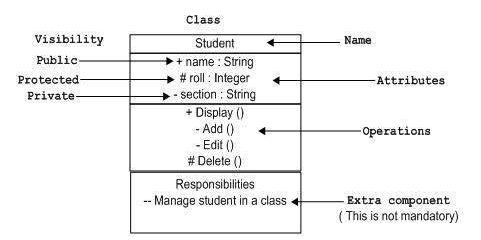
\includegraphics{figures/classDiagram}
	\caption{Schemat diagramu klasy \cite{learnUml}}
	\label{fig:classDiagram}
\end{figure}

\section{Klasa abstrakcyjna}
Na rys. \ref{fig:abstractClassDiagram} przedstawiono schemat wypełniania diagramu 
klasy abstrakcyjnej.
\begin{figure}[H]
	\centering
	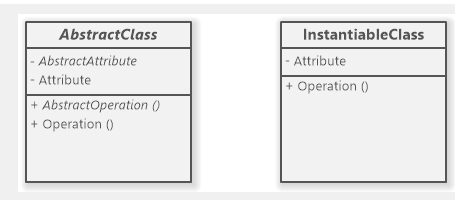
\includegraphics{figures/abstractClassDiagram.png}
	\caption{Schemat diagramu klasy abstrakcyjnej \cite{abstractClass}}
	\label{fig:abstractClassDiagram}
\end{figure}



\chapter{Association vs Aggregation vs Composition}
\section{Rodzaje zależności między klasami}
W UML możemy przedstawić zależności między klasami. Wyróżniamy trzy podstawowe:
\begin{enumerate}
	\item Asocjacje (association)
	\item Agregat (aggregation)
	\item Kompozycja (composition)
\end{enumerate}
Zależności te i sposób i oznaczania na schematach pokazano na rys.
\ref{fig:association}.
\begin{figure}[H]
	\centering
	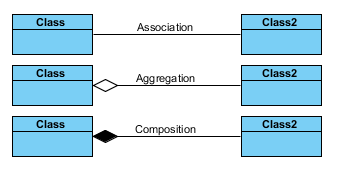
\includegraphics{figures/association}
	\caption{Sposoby oznaczania zależności między klasami w UML \cite{association}}
	\label{fig:association}
\end{figure}


\section{Asocjacja}
Asocjacja występuje gdy dwie klasy muszą się ze sobą komunikować. Asocjacja oznaczana
jest przez połączenie dwóch diagramów klas za pomocą linii. Dana klasa może komunikować
się z wieloma obiektami danego typu co oznaczamy przez dopisanie \verb+1...*+ 
(rys. \ref{fig:oneToMany}).
\begin{figure}[H]
	\centering
	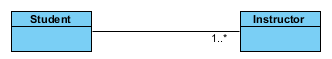
\includegraphics{figures/oneToMany}
	\caption{Przykład asocjacji i sposób oznaczania komunikowania się
	z wieloma obiektami danej klasy - student ma wielu instruktorów \cite{association}} 
	\label{fig:oneToMany}
\end{figure}

\section{Agregacja i kompozycja}
Agregacja i kompozycja to szczególne rodzaje asocjacji. Poniżej przedstawiono definicje:
\begin{itemize}
	\item Agregacja - oznacza związek, w którym potomek może istnieć niezależnie od rodzica. 
		Przykład: Klasa (rodzic) i Uczeń (dziecko). Usunięcie klasy nie powoduje
		usunięcia klasy Uczeń.
		\item Kompozycja - oznacza relację, w której dziecko nie może istnieć 
			niezależnie od rodzica. Przykład: Dom (rodzic) i Pokój (dziecko). 
			Pokoje nie istnieją oddzielnie od domu.
\end{itemize}

\section{Przykłady kompozycji i agregacji}
W przypadku kompozycji powinniśmy być bardziej szczegółowi i używać linku 
do kompozycji w przypadkach, w których oprócz częściowej relacji między klasą A i 
klasą B – istnieje silna zależność cyklu życia między nimi, 
co oznacza, że po usunięciu klasy A usuwana jest również klasa B w rezultacie.
Przykład kompozycji pokazano na rys. \ref{fig:composition}.
\begin{figure}[H]
	\centering
	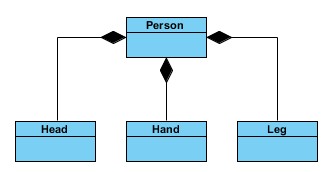
\includegraphics{figures/composition}
	\caption{Przykład kompozycji (composition) \cite{association}}
	\label{fig:composition}
\end{figure}

W przypadku agregacji należy zauważyć, że agregacja w żaden sposób nie stwierdza, 
że klasa A jest właścicielem klasy B ani że istnieje relacja rodzic-dziecko (gdy
rodzic jest usunięty wszystkie jego elementy potomne są w rezultacie usuwane) 
między nimi. Właściwie wręcz przeciwnie! Łącze agregacji jest zwykle używane
do podkreślenia, że instancja klasy A nie jest wyłącznym kontenerem instancji 
klasy B, ponieważ w rzeczywistości ta sama instancja klasy B ma inny kontener (kontenery).
Przykład agregacji pokazano na rys. \ref{fig:aggregation}.
\begin{figure}[H]
	\centering
	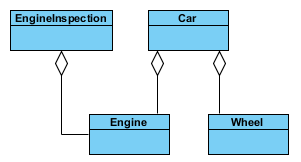
\includegraphics{figures/aggregation}
	\caption{Przykład agregacji (aggregation) \cite{association}}
	\label{fig:aggregation}
\end{figure}

\section{Dziedziczenie}

Dodatkowo możemy oznaczyć, że dana klasa dziedziczy od innej co jest pokazane
na rys. \ref{fig:inheritance}.
\begin{figure}[H]
	\centering
	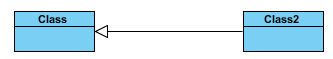
\includegraphics{figures/inheritance}
	\caption{Oznaczania dziedziczenia w UML \cite{association}}
	\label{fig:inheritance}
\end{figure}
Przykład dziedziczenia pokazano na rys. \ref{fig:inheritanceExample}.
\begin{figure}[H]
	\centering
	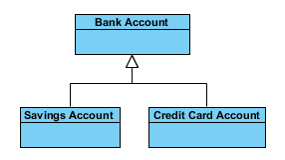
\includegraphics{figures/inheritanceExample}
	\caption{Przykład oznaczenia dziedziczenia w UML \cite{association}}
	\label{fig:inheritanceExample}
\end{figure}

\section{Podsumowanie}
Podsumowując, asocjacja jest bardzo ogólnym terminem używanym do reprezentowania, 
kiedy jedna klasa korzysta z funkcjonalności zapewnianych przez inną klasę. 
Mówimy, że jest to kompozycja, jeśli jeden obiekt klasy nadrzędnej posiada inny 
obiekt klasy podrzędnej i ten obiekt klasy podrzędnej nie może sensownie 
istnieć bez obiektu klasy nadrzędnej. Jeśli tak, to nazywa się to Agregacją.

W C++ z agregacją (diament nie wypełniony) mamy zwykle do czynienia, gdy 
klasa zawiera inny obiekt przez referencję lub wskaźnik. Kompozycja
(diament wypełniony) zachodzi zwykle, gdy dana klasa zawiera obiekt
przez wartość \cite{pointerToClass}.


\addcontentsline{toc}{chapter}{Bibliografia}
\bibliographystyle{plain}
\bibliography{UMLrefs}
\lstlistoflistings

\end{document}
